% ADD/REMOVE THE 'answers' OPTION TO INCLUDE/SUPPRESS SOLUTIONS
% \documentclass[11pt,addpoints]{exam}
\documentclass[11pt,addpoints,answers]{exam}

\newcommand{\hwnum}{1}
\newcommand{\duedate}{September 9}

% In order to compile this file you will need to get 'header.tex'
% and make the line below point to the appropriate file path
\RequirePackage{microtype}
\RequirePackage{mathtools}
\RequirePackage{amsthm}
\RequirePackage{amssymb}
\RequirePackage{xspace}
\RequirePackage[shortlabels]{enumitem}
\RequirePackage{xcolor}
\RequirePackage{hyperref}
\RequirePackage[capitalize,nameinlink,noabbrev]{cleveref} % must load after hyperref
\usepackage{fvextra} % To use Verbatim
\usepackage{diagbox} % For diagbox
\RequirePackage[boxed]{algorithm}
\RequirePackage[noend]{algpseudocode}
\RequirePackage{tikz}
\usetikzlibrary{arrows,automata,positioning}

\hypersetup{breaklinks=true,
    colorlinks=true,
    linkcolor=blue,
    filecolor=blue,
    citecolor=blue,
    urlcolor=blue}

\algrenewcommand{\algorithmiccomment}[1]{\texttt{//} #1}
\algrenewcommand\algorithmicrequire{\textbf{Input:}}
\algrenewcommand\algorithmicensure{\textbf{Output:}}


% allow cleveref to label and reference enumerables defined in the exam class.
% these automatically define corresponding \Crefname as well.

% https://tex.stackexchange.com/questions/126020/cleveref-doesnt-use-correct-capitalized-name-if-used-with-amsthm
\makeatletter
\if@cref@capitalise
\crefname{question}{Question}{Questions}
\Crefname{partno}{Part}{Parts}
\crefname{subpart}{Subpart}{Subparts)}
\crefname{subsubpart}{Subsubpart}{Subsubparts}
\else
\crefname{question}{question}{questions}
\crefname{partno}{part}{parts}
\crefname{subpart}{subpart}{subparts}
\crefname{subsubpart}{subsubpart}{subsubparts}
\fi
\makeatother

% numeric sets in "blackboard" font

\newcommand{\N}{\mathbb{N}}
\newcommand{\Z}{\mathbb{Z}}
\newcommand{\R}{\mathbb{R}}
\newcommand{\Q}{\mathbb{Q}}
\newcommand{\C}{\mathbb{C}}
\newcommand{\Prop}{\mathbb{P}}

% paired delimiters

\DeclarePairedDelimiter\abs{\lvert}{\rvert}
\DeclarePairedDelimiter\length{\lVert}{\rVert}
\DeclarePairedDelimiter\norm{\lVert}{\rVert}
\DeclarePairedDelimiter\parens{(}{)}
\DeclarePairedDelimiter\tuple{(}{)}
\DeclarePairedDelimiter\brackets{[}{]}
\DeclarePairedDelimiter\floor{\lfloor}{\rfloor}
\DeclarePairedDelimiter\ceil{\lceil}{\rceil}
\DeclarePairedDelimiter\round{\lfloor}{\rceil}
\DeclarePairedDelimiter\set{\{}{\}}
\DeclarePairedDelimiter\inner{\langle}{\rangle}

\newcommand{\bit}{\set{0,1}}

% asymptotics

\DeclareMathOperator{\Otil}{\tilde{O}}
\DeclareMathOperator{\poly}{poly}
\DeclareMathOperator{\polylog}{polylog}
\DeclareMathOperator{\negl}{negl}

% algorithms

\newcommand{\algo}[1]{\textsc{#1}}

\newcommand{\memo}{\text{memo}}
\newcommand{\tabl}{\text{table}}
\newcommand{\backtrack}{\text{backtrack}}

\newcommand{\ALG}{\text{ALG}}
\newcommand{\OPT}{\text{OPT}}
\newcommand{\weight}{\text{weight}}
\newcommand{\val}{\text{value}}

% computability

% named language
\newcommand{\lang}[1]{L_{\text{#1}}}
% computational problem
\newcommand{\cproblem}[1]{\ensuremath{\text{#1}}\xspace}
% class of languages
\newcommand{\class}[1]{\ensuremath{\mathsf{#1}}\xspace}

\newcommand{\qst}{q_{\text{start}}}
\newcommand{\qacc}{q_{\text{acc}}}
\newcommand{\qrej}{q_{\text{rej}}}

\newcommand{\Lbarber}{\lang{BARBER}}
\newcommand{\atm}{\lang{ACC}}
\newcommand{\htm}{\lang{HALT}}
\newcommand{\ehtm}{\lang{$\varepsilon$-HALT}}
\newcommand{\eqtm}{\lang{EQ}}
\newcommand{\etm}{\lang{$\emptyset$}}
\newcommand{\epstm}{\lang{$\set{\varepsilon}$}}
\newcommand{\Lprop}{\lang{$\Prop$}}
\newcommand{\LSigmastar}{\lang{$\Sigma^*$}}

% complexity

\newcommand{\yes}{\ensuremath{\text{YES}}}
\newcommand{\no}{\ensuremath{\text{NO}}}

\newcommand{\DTIME}{\class{DTIME}}
\renewcommand{\P}{\class{P}}
\newcommand{\NP}{\class{NP}}
\newcommand{\NPH}{\class{NPH}}
\newcommand{\NPC}{\class{NPC}}
\newcommand{\coNP}{\class{coNP}}

\newcommand{\MAZE}{\cproblem{MAZE}}
\newcommand{\PALINDROME}{\cproblem{PALINDROME}}
\newcommand{\TSP}{\cproblem{TSP}}
\newcommand{\SAT}{\cproblem{SAT}}
\newcommand{\CSAT}{\cproblem{CSAT}}
\newcommand{\TSAT}{\cproblem{3SAT}}
\newcommand{\VC}{\cproblem{VERTEX-COVER}}
\newcommand{\DS}{\cproblem{DOMINATING-SET}}
\newcommand{\SC}{\cproblem{SET-COVER}}
\newcommand{\HC}{\cproblem{HAMCYCLE}}
\newcommand{\HP}{\cproblem{HAMPATH}}
\newcommand{\AHP}{\cproblem{ANYHAMPATH}}
\newcommand{\IS}{\cproblem{IS}}
\newcommand{\CLIQUE}{\cproblem{CLIQUE}}
\newcommand{\SSUM}{\cproblem{SUBSET-SUM}}
\newcommand{\KNAPSACK}{\cproblem{KNAPSACK}}
\newcommand{\MAXCUT}{\cproblem{MAX-CUT}}

% randomness

\DeclareMathOperator*{\Var}{Var}
\DeclareMathOperator*{\Ex}{\mathbb{E}}

\newcommand{\RP}{\class{RP}}
\newcommand{\coRP}{\class{coRP}}
\newcommand{\BPP}{\class{BPP}}
\newcommand{\ZPP}{\class{ZPP}}
\newcommand{\BQP}{\class{BQP}}

%%% misc

\newcommand{\eps}{\varepsilon}

%%% theorems

\theoremstyle{plain}            % following are "theorem" style

\newtheorem{theorem}{Theorem}
\newtheorem{lemma}[theorem]{Lemma}
\newtheorem{corollary}[theorem]{Corollary}
\newtheorem{proposition}[theorem]{Proposition}
\newtheorem{claim}[theorem]{Claim}
\newtheorem{fact}[theorem]{Fact}
\newtheorem{openproblem}[theorem]{Open Problem}

\theoremstyle{definition}       % following are def style

\newtheorem{definition}[theorem]{Definition}
\newtheorem{conjecture}[theorem]{Conjecture}
\newtheorem{protocol}[theorem]{Protocol}
\newtheorem{exercise}[theorem]{Exercise}

\theoremstyle{remark}           % following are remark style

\newtheorem{example}[theorem]{Example}
\newtheorem{remark}[theorem]{Remark}
\newtheorem{note}[theorem]{Note}

%%% for homework and section notes

\newcommand{\commonheader}[2]{
    \pagestyle{headandfoot}
    \setlength{\headheight}{26pt}
    \setlength{\headsep}{16pt}

    \header
        {\small{\textbf{EECS 376: Foundations of Computer Science}} \\ \footnotesize{\textbf{University of Michigan, Fall 2026}}}
        {#1}
        {#2}

    \firstpageheadrule
    \runningheadrule

    \footer
        {}
        {\thepage}
        {}
}

\newcommand{\hwheader}{
    \commonheader
        {\Large \textbf{Homework \hwnum}}
        {\small \textbf{Due 8:00pm, \duedate\\ {\tiny(accepted until 10:00 pm, no credit after)}}}
}

\newcommand{\hwslnheader}{
    \commonheader
    	{}
        {\Large \textbf{Solutions to Homework \hwnum}}
    \printanswers
}

\newcommand{\notesheader}{
    \commonheader
    	{}
        {\Large \textbf{Discussion Notes \sectionnum}}
}

\newcommand{\practiceheader}{
    \commonheader
    	{}
        {\Large \textbf{Discussion Worksheet \sectionnum}}
}

\newcommand{\practiceslnheader}{
    \commonheader
    	{}
        {\Large \textbf{Solutions to Discussion Worksheet \sectionnum}}
}

\newcommand{\reviewheader}{
    \commonheader 
    \smallskip
    	{}
        {\Large \textbf{Midterm Review Notes}}
}

\newcommand{\hwpreface}{

\noindent This homework has \numquestions\ questions, for a total of \numpoints\ points and \numbonuspoints\ extra-credit points.

\noindent Unless otherwise stated, each question requires \emph{clear}, \emph{logically correct}, and \emph{sufficient} justification to convince the reader.

\noindent We strongly encourage you to typeset your solutions in \LaTeX.

}

\newcommand{\hint}[1]{
\emph{Hint}: #1
}

% exam class setup
\pointsinmargin
\pointpoints{pt}{pts}
\bonuspointpoints{EC pt}{EC pts}
\marginpointname{ \points}
\marginbonuspointname{ \bonuspoints}
 

\ifprintanswers
\hwslnheader   % header for solutions
\else
\hwheader   % header for homework
\fi

\begin{document}

\hwpreface

\begin{questions}

  \addtocounter{question}{-1}
  \question[0] \textbf{Before you start; before you submit.}
  
  \begin{parts} 
    \part Before starting this assignment, carefully read \href{https://drive.google.com/file/d/1nxOmNy9oxfo0jU2u4vLkcwV8fCBEfPZg/view?usp=drive_link}{Handout 1} (Running Times and Asymptotics) and the ``Good Writing'' section of \href{https://drive.google.com/file/d/1r28RQOszVmRXKwOpQtyLFu0c3HYMnxyl/view?usp=drive_link}{Handout 2} (the induction section is optional but recommended), and apply them to your work.

    \part If applicable, state the name(s) and uniqname(s) of your collaborator(s).

    \begin{solution}
       
    \end{solution}

  \end{parts}

  \bonusquestion \textbf{\LaTeX\ (optional extra credit).} 

We (along with the rest of the math-writing world) use \LaTeX\ to write all homeworks and exams. Throughout the semester, we strongly encourage you to write all of your homework solutions in \LaTeX\ too. This extra credit problem will give you some practice with \LaTeX.

To compile \LaTeX\ code, you can use the website \url{overleaf.com}, or download a \LaTeX\ editor of your choice. To compile each of the EECS 376 homework assignments in \LaTeX\ you will also need to upload the provided \texttt{header.tex} file into your project.

\LaTeX\ is \emph{not} a ``what you see is what you get'' word-processing software like you may be accustomed to (Word, Google Docs, etc.).
Instead, a \LaTeX\ document is a \emph{program} that describes the desired output, and is \emph{compiled} into a human-readable format.



Here are some good resources about \LaTeX\ practices:
\begin{itemize}[itemsep=0pt]
\item \href{https://www.gleave.me/post/latex-design-patterns/}{Writing Beautifully in \LaTeX},
\item \href{https://tug.ctan.org/info/short-math-guide/short-math-guide.pdf}{Short Math Guide for \LaTeX},
\item \href{https://chenfuture.wordpress.com/2009/02/07/dos-and-donts-when-typesetting-a-document/}{DOs and DON'Ts when typesetting a document}.
\end{itemize}
  
To receive the extra credit points, you must typeset this \textbf{entire} assignment in \LaTeX, and typeset the two snippets of text given in parts (a) and (b) in \LaTeX.
\textbf{Put your solution to this problem in the \texttt{Verbatim} environment as follows so that we can see the \LaTeX~source code in your compiled PDF} (do not use the \texttt{Verbatim} environment for the rest of the assignment): 

\begin{Verbatim}[breaklines, breaksymbol=]
    This text is in the \texttt{Verbatim} environment. \emph{This} word is italicized. Here is some math: $1+1=2$.
\end{Verbatim}

Here are some examples of  \LaTeX\ syntax you may need:
      \begin{itemize}
          \item In-line math
          \item Less-than-or-equal-to symbol
          \item Quote marks
          \item Bulleted lists
        \item Display math
        \item The \texttt{algorithmic} environment
    \end{itemize}
   You may copy and modify the source code of this document (e.g.~part (b) asks you to write an algorithm in \LaTeX, and other problems in this document already contain algorithms). You may also use the Internet to search for \LaTeX\ syntax.

\ifprintanswers
\else
\newpage
\fi

  \begin{parts}
      \bonuspart[5] The following snippet is about some key features of the big-O notation extracted from \href{https://drive.google.com/file/d/1s8EuLp-75kDk3tE4_j18htpUnG4diVoq/view?usp=drive_link}{Handout 1}.
      \begin{center}
        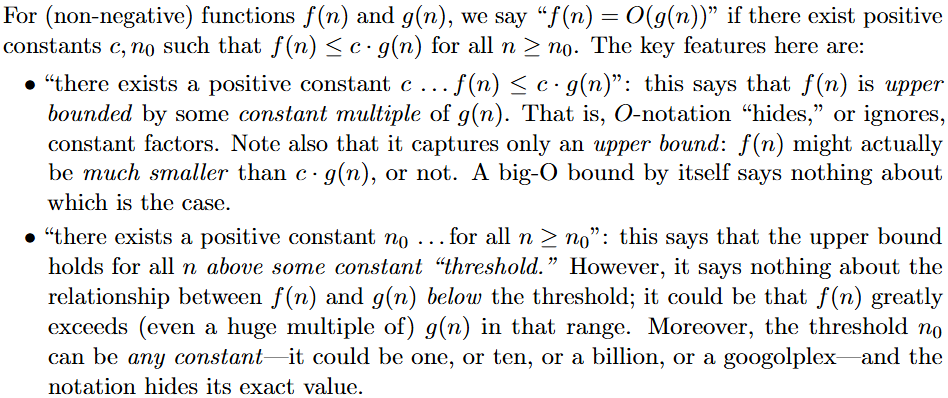
\includegraphics[width=\linewidth]{asymp.png}
      \end{center}


      \begin{solution}
      \end{solution}

    \bonuspart[5] The following snippet is about \href{https://en.wikipedia.org/wiki/Fibonacci_sequence}{Fibonacci numbers}. 
      \begin{center}
        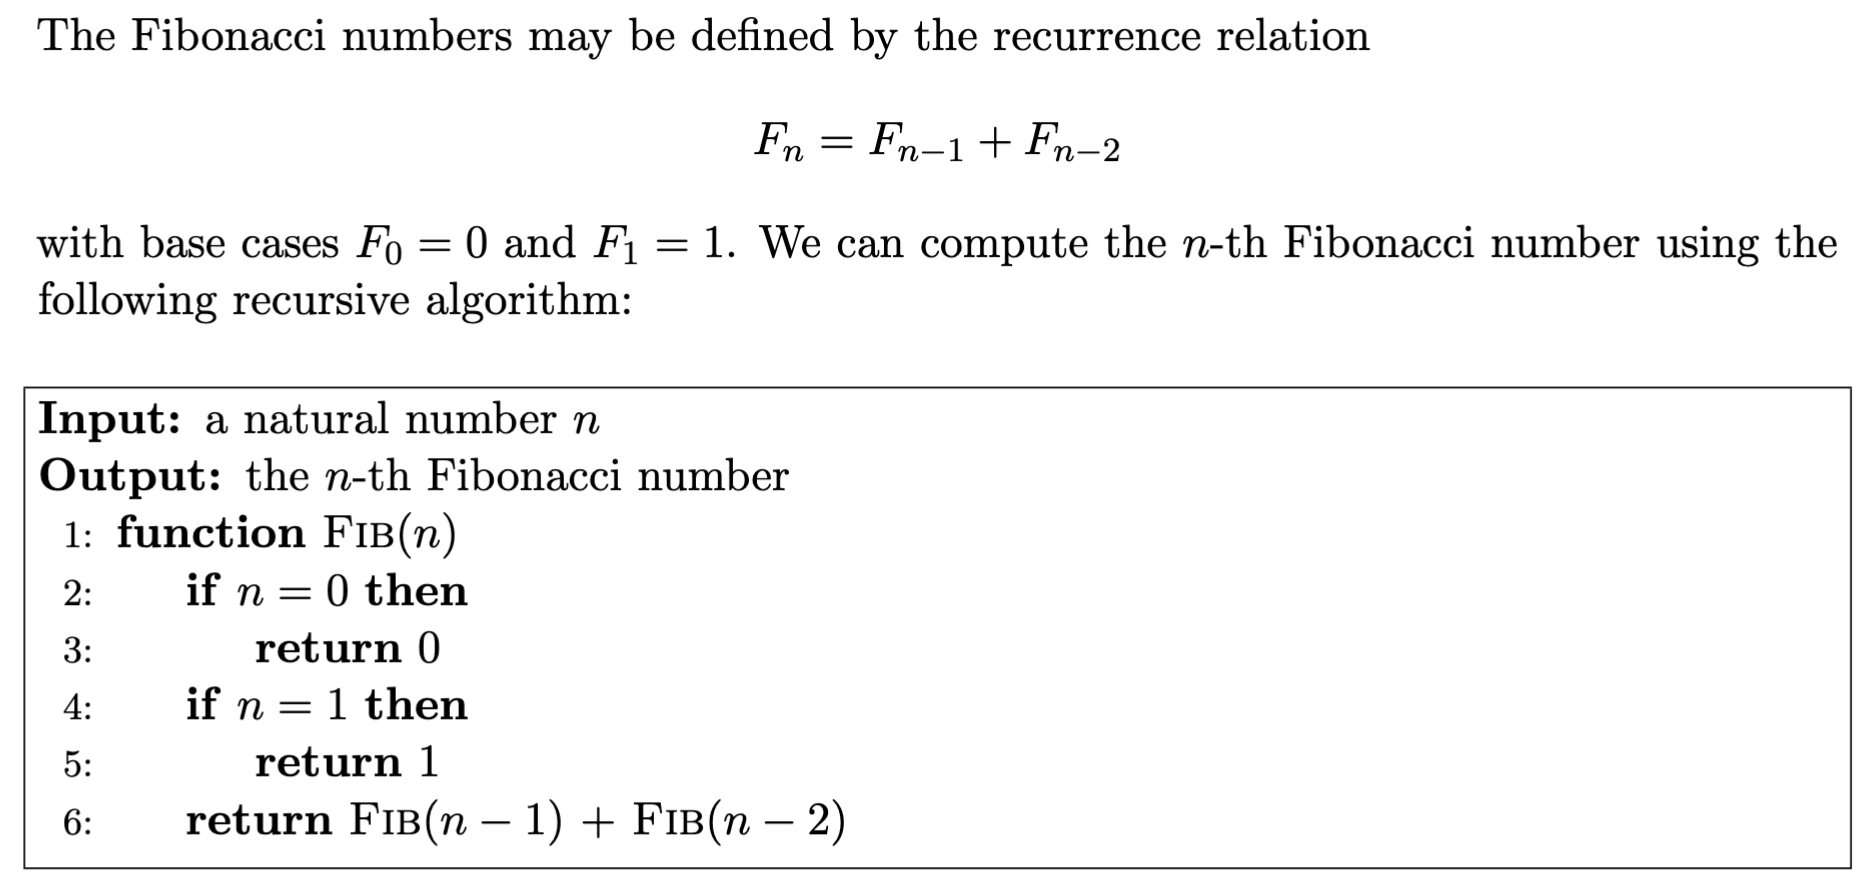
\includegraphics[width=\linewidth]{fib.png}
      \end{center}
    



    \begin{solution}
    \end{solution}

  \end{parts}

\ifprintanswers
\else
\newpage
\fi

 \question \textbf{Properties of logarithms.}
 
  The objective of this problem is to recall some important properties of logarithms that we'll use throughout the course.
  First recall the following properties of exponentiation for any real numbers $b, x, y$, assuming that $b \neq 0$:
  \begin{description}
  \item[P1:] $(b^x)^y = b^{xy}$
  \item[P2:] $b^x = b^y$ if and only if $x = y$, additionally assuming that $b \neq 1$.
  \end{description}

  Now, for positive real numbers $b \neq 1$ and~$x$, the definition of the base-$b$ logarithm is:
  \begin{description}
  \item[D1:] $y = \log_b x$ is the unique real number for which $b^y = x$.
    That is, it satisfies the identity $b^{\log_{b} x} = x$.
  \end{description}
  
  Combining D1 with P2, we see that $x=y$ if and only if $\log_{b} x = \log_{b} y$ (assuming that $b,x,y$ are positive and $b \neq 1$).
  So, equality is preserved by taking logarithms or exponentials (with the same base) on both sides of an equation, assuming the hypotheses are met. You may use this fact in your solutions.

  Prove each of the following properties of logarithms, for any positive real numbers (not necessarily integers) $a, b, c, n$ where $b, c \neq 1$.
  Cite definition D1 and properties P1 and P2 where you use them; you may also use (with citation) the results of previous parts of the problem. 
  Do not use any other assumptions about, or properties of, logarithms and exponentials.

  For reference, we have provided a solution to the first part, which you can use as a model for later solutions.
   
  \begin{parts}
    \part[0] $\log_{b} (a^{n}) = n \log_{b} a$.
    (Be careful: $n$ is not necessarily an integer) \label{parta}
    
    \begin{solution}


      By P2, the statement we want to prove is equivalent to $b^{\log_{b} (a^{n})} = b^{n \log_{b} a}$ (since $b \neq 1$).
      By D1, the left-hand side is equal to $a^{n}$, so it suffices to prove that $a^{n} = b^{n \log_{b} a}$.
      Indeed,
      \[ b^{n \log_{b} a} = (b^{\log_{b} a})^{n} = a^{n} , \]
      where the first equality is by P1, and the second equality is by D1.

      (As a remark, this proof does not rely on the assumption that~$n$ is positive, so the statement holds even more generally for any real number~$n$.
      However, later parts require~$n$ to be positive.)
    \end{solution}
                
    \part[3] $\log_{b} a = \frac{\log_{c} a}{\log_{c} b}$.
    (This is sometimes called the ``change-of-base theorem,'' because it lets us change the base of the logarithm by dividing by an appropriate factor.
    Note that $\log_{c} b \neq 0$ because $b \neq 1$, so the division is well defined.)

    \begin{solution}
    \end{solution}

    

     \part[3]$a^{\log_{b} n} = n^{\log_{b} a}$.  (This is sometimes called the ``log-switching theorem'' since it says that we can ``switch'' $a$ and $n$.)

     \begin{solution}
     \end{solution}
    
    \part[3] The ratio $\frac{\log_{b} n}{\log_{c} n}$ (for $n \neq 1$) depends only on~$b$ and~$c$, not~$n$.

    This implies that we can often omit the (constant) base when writing logarithms in asymptotic notation, e.g., we can write $O(\log n)$ instead of $O(\log_2 n)$, because $O(\cdot)$ hides constant factors that do not depend on~$n$.
    However, we cannot omit the base when the logarithm appears in the exponent, as in $O(3^{\log_2 n})$.

    \begin{solution}
    \end{solution}


  \end{parts}


  \question \textbf{Welcome to EECS 376!}


To express our excitement for the start of EECS 376, we present an algorithm that prints \texttt{"Welcome to EECS 376!"} multiple times, based on input parameter $n$.

\begin{minipage}{\linewidth}
\begin{algorithm}[H]
      \begin{algorithmic}[1]
        \Require{positive integer $n$ represented in binary}
        \Function{\text{Welcome}}{$n$} 
        \For{$i = 1, 2, \dots, n$}
            \For{$j = 1, 2, \dots, i$}            
            \State {\Call{Print}{\texttt{"Welcome to EECS 376!"}}}
            \EndFor
        \EndFor
        \EndFunction
      \end{algorithmic}
\end{algorithm}
\end{minipage}

\begin{parts}

    \part[4] Give the \emph{tightest correct asymptotic} (big-$O$) bound, as a function of~$n$, on the worst-case running time of the \textsc{Welcome}($n$) algorithm. 

    \begin{solution}
    \end{solution}

    \part[4] Let $s$ be the input size of the integer $n$, i.e., the number of bits needed to represent $n$ in binary. Give the tightest correct asymptotic (big-$O$) bound, as a function of~$s$, on the worst-case running time of the \textsc{Welcome} algorithm. State whether or not the algorithm is \emph{efficient}, i.e., runs in at most polynomial time with respect to the input size $s$. \label{3c}
    
    % \emph{Reminder}: The input size of an integer is defined as the number of bits needed to represent it in binary.

    \begin{solution}
    \end{solution}

    \part [4] Does your answer in \cref{3c} change if $n$ is represented in decimal (base-10) instead? That is, let $s'$ be the input size of the integer $n$, i.e., the number of digits needed to represent $n$ in base-10. Give the tightest correct asymptotic (big-$O$) bound, as a function of~$s'$, on the worst-case running time of the \textsc{Welcome} algorithm. State whether or not the algorithm is \emph{efficient}, i.e., runs in at most polynomial time with respect to the input size $s'$.


    \begin{solution}
    \end{solution}

      \part [4] Now consider a different algorithm $\mathcal{A}$ that takes an input an integer $n$ and has worst-case running time $O(\log n)$. 
      
      Suppose $n$ is represented in binary and let $s$ be the input size (number of bits in $n$). Give the tightest correct asymptotic (big-$O$) bound, as a function of~$s$, on the worst-case running time of algorithm $\mathcal{A}$. State whether or not the algorithm is \emph{efficient}.
      
      Does your answer change if $n$ is represented in base-10 instead? That is, let $s'$ be the input size (number of digits needed to represent $n$ in base-10). Give the tightest correct asymptotic (big-$O$) bound, as a function of~$s'$, on the worst-case running time of algorithm $\mathcal{A}$. State whether or not the algorithm is \emph{efficient}.

\begin{solution}
   \end{solution}
    
\end{parts}

 \question \textbf{Practice with asymptotics (``big-Oh, big-Omega, big-Theta'').}

  Let $f(n)$ and $g(n)$ be positive functions.
  Recall that $f(n) = O(g(n))$ if there exist constants $c, n_0 > 0$ such that $f(n) \leq c \cdot g(n)$ for all $n \geq n_0$.

  \begin{itemize}
    \item In words, this says: ``$f(n)$ is \emph{at most} (or: is \emph{upper-bounded by}) a \emph{constant multiple} of $g(n)$, for \emph{all large enough}~$n$.''
    (``All large enough~$n$'' refers to the clause ``all $n \geq n_{0}$'', i.e., all~$n$ beyond some fixed threshold.)

   \item It can be shown that:
    \begin{enumerate}
        \item If $\lim_{n \to \infty} \frac{f(n)}{g(n)}$ is finite, $f(n) = O(g(n))$ is true.
        \item If $\lim_{n \to \infty} \frac{f(n)}{g(n)}$ is infinite, $f(n) = O(g(n))$ is false.
        \item If $\lim_{n \to \infty} \frac{f(n)}{g(n)}$ does not exist, we cannot conclude whether $f(n) = O(g(n))$ is true or false. For example, for $f(n) = \abs{\sin(n)}$ and $g(n)=2$ the limit does not exist, but $f(n)=O(g(n))$.
    \end{enumerate}
  \end{itemize}

   Similarly, $f(n) = \Omega(g(n))$ if there exist constants $c, n_{0} > 0$ such that $f(n) \geq c \cdot g(n)$ for all $n \geq n_{0}$.
  \begin{itemize}
      \item In words, this says that ``$f(n)$ is \emph{at least} (or: is \emph{lower-bounded by}) a positive-constant multiple of $g(n)$, for all large enough~$n$.''
      \item It can be shown that:
      \begin{enumerate}
          \item If $\lim_{n \to \infty} \frac{f(n)}{g(n)}$ is greater than zero (including infinity), $f(n) = \Omega(g(n))$ is true.
          \item If $\lim_{n \to \infty} \frac{f(n)}{g(n)}$ is zero, $f(n) = \Omega(g(n))$ is false.
          \item If $\lim_{n \to \infty} \frac{f(n)}{g(n)}$ does not exist, we cannot conclude whether $f(n) = \Omega(g(n))$ is true or false. 
      \end{enumerate}
      % When $\lim_{n \to \infty} \frac{f(n)}{g(n)}$ exists or is infinite, $f(n) = \Omega(g(n))$ if and only if the limit is greater than zero (including infinite).
  \end{itemize}
  
  
  Moreover, it can be seen that $f(n) = \Omega(g(n))$ is equivalent to $g(n) = O(f(n))$, since $f(n) \geq c \cdot g(n)$ if and only if $g(n) \leq (1/c) \cdot f(n)$, and~$c$ is a positive constant if and only if $1/c$ is a positive constant.
  
  Finally, $f(n) = \Theta(g(n))$ if both $f(n) = O(g(n))$ and $f(n) = \Omega(g(n))$.

  For the following pairs of functions, state, with rigorous proof, whether or not each of the following hold: $f(n) = O(g(n))$, $f(n) = \Omega(g(n))$, $f(n) = \Theta(g(n))$.

  \hint{You might find L'H\^{o}pital's Rule useful, which says (in particular): if $f(n),g(n)$ are differentiable, $g'(n) \neq 0$ for all large enough~$n$, and $\lim_{n \to \infty} g(n) = \infty$, then $\lim_{n \to \infty} \frac{f(n)}{g(n)} = \lim_{n \to \infty} \frac{f'(n)}{g'(n)}$ whenever the latter limit exists.
  (Here~$f'$ and~$g'$ are respectively the derivatives of~$f$ and~$g$.)
  You may use a calculator or computer to calculate derivatives.}

  \begin{parts}
    \part[3] $f(n) = \log_{2}(n^3)$, $g(n) = \log_{5}(n^{1/8})$.

    Optional ungraded challenge: generalize to similar-looking $f$ and $g$, beyond specific constant bases and exponents.
    
    \begin{solution}
    \end{solution}

    \part[4] $f(n) = (376 + \sin(n)) \cdot n$, $g(n) = 203 n$.

    Optional ungraded challenge: generalize to similar-looking $f$ and $g$, beyond specific constant coefficients or exponents.
    
    \begin{solution}
    \end{solution}

    \part[6] $f(n) = n^{3} \cdot 2^{3n}$, $g(n) = 3^{2n}$.
    
    Optional ungraded challenge: generalize to similar-looking $f$ and $g$, beyond specific constants in the bases and exponents.

    \begin{solution}
    \end{solution}

  \end{parts}


 
  \question \textbf{Prof. Upsilon and their oopsie claims.}

  
  Prof.~$\Upsilon$ is an absent-minded computer scientist, known for their occasional ``oopsie" moments. Recently, Prof.~$\Upsilon$ came up with three algorithms with the following running times:  

  \begin{itemize}
      \item Algorithm $X$ has worst-case running time $T_{X}(n) = O(n^2)$
      \item Algorithm $Y$ has worst-case running time $T_{Y}(n) = \Theta(n \log n)$
      \item Algorithm $Z$ has worst-case running time $T_{Z}(n) = \Theta(n)$
  \end{itemize}

  Recall that \emph{worst-case} running time of an Algorithm $A$ means the \emph{maximum} number of steps for which $A$ runs, over all possible inputs of size~$n$. %$T_{X}(n)$ is the \emph{maximum} number of steps for which X runs, taken over all inputs of size~$n$ (and similarly for $T_{Y}, T_{Z}$).

  Now, Prof.~$\Upsilon$ has made a series of claims about these algorithms.  State, with proof, whether Prof.~$\Upsilon$'s claim is necessarily true, necessarily false, or not necessarily either based on the given information. If it is not necessarily either, give an example when it is true and an example when it is false. For instance, such an example could be of the form: ``Suppose Algorithm $Y$ takes time $8n\log n$ for some inputs and time $4n$ for the remaining inputs.''
  
  \begin{solution}
  \end{solution}


  \begin{parts}
    \part[4] ``Algorithm $Y$ has running time $O(n^2)$.''

  \begin{solution}
  \end{solution}

    \part[6] ``On every sufficiently large input, Algorithm $Z$ runs faster than Algorithm $Y$.''
   \begin{solution}
    \end{solution}

    \part[6] ``For all large enough $n$, there is an input of size $n$ for which $Y$ runs faster than $X$.''
    \begin{solution}
    \end{solution}

    \part[6] ``For all large enough $n$, there is an input of size $n$ for which $Z$ runs faster than $Y$.''

    \begin{solution}
    \end{solution}
\end{parts}

    \question \textbf{Set of proofs by contra-.}
    
    Recall that a \emph{set} is a collection of distinct elements. Below are some important set notations:
    \begin{itemize}
        \item \textbf{Elements of a set:} $x \in A$ means $x$ is an element of set $A$. 
        \item \textbf{Complement of a set:\footnote{In some texts, you may encounter notations like $A^C$, $A^\complement$, $A'$, etc. to refer to the complement of $A$.}} $\overline{A}$ refers to the set of all elements in the universal set $U$ that are not in $A$.
        \item \textbf{Subset:} $A \subseteq B$ means every element of $A$ is also an element of $B$. 
        \item \textbf{Intersection of sets:} $A \cap B$ is the set of elements that are in both $A$ and $B$. 
        \item \textbf{Union of sets:} $A \cup B$ is the set of elements that are in $A$, in $B$, or in both.
        \item \textbf{Set difference:} $A \setminus B$ is the set of elements that are in $A$ but not in $B$. We can also write it as $A \cap \overline{B}$.
    \end{itemize}

    \begin{parts}
        \part [4] Recall the transitive property of the subset relation: 
        \begin{quote}
            If $A \subseteq B$ and $B \subseteq C$, then $A \subseteq C$.
        \end{quote}
        Prove the above property by contradiction. 

        \begin{solution}
        \end{solution}

        \part [4] Recall the DeMorgan's Law, which says: 
        \begin{quote}
            If $x \in \overline{A \cap B}$, then  $x \in \overline{A} \cup \overline{B}$.
        \end{quote}
        State the contrapositive of the statement. Then, prove the contrapositive.

        \begin{solution}
        \end{solution}
        
    \end{parts}

    \question \textbf{Requirements for the potential method.}

  Recall that the potential method requires several properties to hold in order to prove that a given process must eventually halt, within a certain number of ``time units.''
  These requirements include (but are not limited to):
  \begin{enumerate}[itemsep=0pt]
  \item the potential cannot go below some fixed lower bound; or if it does, the process must immediately halt.
  \label{lower-bound}
  
  \item the potential must \emph{decrease by (at least) some fixed positive amount} with each time unit.\label{decrease}
  \end{enumerate}

  For each of the following processes and candidate potential functions, state with justification whether they satisfy each of the above properties.
  If not, either describe an alternative potential function that does satisfy both properties (and allows us to conclude that the process must halt), or briefly explain why the process might not ever halt (and hence there is \emph{no} valid potential function for the process).

  \begin{parts}
    
    \part[4] You take a road trip from Michigan to California, which are about 2360 miles apart.
    On each day, you drive \emph{half} of your remaining distance to California, and then stop to see the sights.
    So, you drive (roughly) 1180 miles on the first day, 590 miles on the second day, 295 miles on the third day, and so forth.
    Define a time unit to be one day of driving, and the potential~$s_{i}$ after~$i$ days of driving to be your remaining distance to California.
    The road trip ends once you reach California.

    \begin{solution}
    \end{solution}
        
    \part[6] You initially have 203 coins lying flat on a table, all showing heads.
    You repeatedly perform the following action: if it is possible to do so, you \emph{must} choose a pair of coins showing heads and turn over \emph{both} of them to show tails.
    Otherwise, you may turn over \emph{any one or two coins} of your choice.
    You continue until no coins are showing heads.
    Define a time unit to be one ``action'' that turns over one or two coins, and the potential~$s_{i}$ to be the number of heads showing after~$i$ actions.

    \begin{solution}
    \end{solution}

    \part[8]
    Consider this process for sorting a given array of~$n$ distinct integers $A[1,\ldots,n]$ in increasing order: repeatedly select any two out-of-order elements (i.e., two elements $A[j]$ and $A[k]$ where $j<k$ but $A[j] > A[k]$) and swap them in the array.
    The process continues until there are no out-of-order elements, in which case the array is then in sorted order.
    Define a time unit to be one swap, and the potential $s_i$ after~$i$ swaps to be the number of array elements that are \emph{not} in the positions they would occupy if the array were sorted.

    \begin{solution}
    \end{solution}
    
  \end{parts}

    
  \question \textbf{Euclid's algorithm, extended.}
  
  Given two integers $x,y$ (that are not both zero), one may wonder what values can be obtained by summing integer multiples of~$x$ and~$y$, i.e., expressed as $ax+by$ for some (not necessarily positive) integers $a,b$.
  It is impossible to obtain any positive integer \emph{smaller} than their GCD $g = \gcd(x,y)$, because $ax+by$ must be divisible by~$g$.
  But, it turns out that the GCD of $x$ and $y$ \emph{can} always be expressed as $ax+by$ for some integers $a,b$; this theorem is known as \emph{B\'{e}zout's identity} (pronounced ``BAY-zoo'').
    
  In this problem, you will modify the standard Euclidean algorithm to output not only $g=\gcd(x,y)$ itself, but also a pair $(a,b)$ of integers for which $ax+by = g$.
  Such integers are called \emph{B\'{e}zout coefficients} for~$x,y$.   (As we will see later, this is very important for cryptography!)
  We give most of the algorithm below:
    
    \begin{minipage}{\linewidth}
      \begin{algorithm}[H]
        \begin{algorithmic}[1]
             \Require{integers $x \geq y\geq 0$, not both zero}
            \Ensure{a triple $(g,a,b)$ of integers where $g = \gcd(x,y) = ax+by$}
            \Statex
            \Function{ExtendedEuclid}{$x,y$}
            \If{$y = 0$} \State \Return $(x,1,0)$
            \Comment{Base case: $1x + 0y = x = \gcd(x,0)$}
            \Else \State Divide $x$ by $y$, writing $x = qy + r$ for integer quotient $q$ and remainder $0\leq r < y$
            \State $(g,a',b') \gets \Call{ExtendedEuclid}{y,r}$
            \State [\textbf{FOR YOU TO DETERMINE:} compute appropriate $a$, $b$]
            \State \Return $(g, a, b)$
            \EndIf
            \EndFunction
        \end{algorithmic}
      \end{algorithm}
    \end{minipage}

  \begin{parts}
  
    \part[6] State what $a$ and $b$ should be on Line 7, and prove that that $ax + by = g$. 

    \emph{Hint}: by recursion/induction, we know that $g = \gcd(y,r)$ and $a'y+b'r = g$.
     
    \begin{solution}
    \end{solution}
    
    \part[8]
    \textbf{Run the Extended Euclid algorithm by hand} to find B\'{e}zout coefficients for the input $(x,y) = (376,203)$, and show that the output is correct.
    (You may use a calculator/computer only for the division steps.)
    Fill in the table below with a `trace' of the execution, i.e., all the variables' values in all the iterations.
    Also include the potential values $s = x+y$, the ratios (as fractions) of potentials $s_{i+1}/s_i$ for adjacent iterations, and Y/N indications of whether $s_{i+1}/s_i \leq 2/3$.

    The entries labeled `input', `division', $s$, and $s_{i+1}/s_i$ should be filled from top to bottom, corresponding to the recursive calls; the `recursive answer' and `output' entries will need to be filled from bottom to top, corresponding to the `post-processing' (Line 7) of each recursive call's results.
    The entries for $a,b$ should match those of $a',b'$ one row above.
    Put~`--' for any entries that are not defined due to the base case. 

  \begin{solution}
      \begin{table}[H]\centering
        \begin{tabular}{r|rr|rr|rr|rr|rrc}
          & \multicolumn{2}{c|}{input} & \multicolumn{2}{|c|}{division} & \multicolumn{2}{|c|}{rec ans} & \multicolumn{2}{|c|}{output} \\
          $i$ & $x$   & $y$  & $q$ & $r$  & $a'$ & $b'$ & $a$ & $b$ & $s$ & $s_{i+1}/s_{i}$ & $\leq 2/3$ ? \\ \hline
          $0$ & $376$ & $203$ &  &  &  &  & &  &  &  & \\
          $1$ &  & &  &  &  &  & &  &  &  & \\
          $2$ &  & &  &  &  &  & &  &  &  & \\
          $\vdots$ &  & &  &  &  &  & &  &  &  & \\
        \end{tabular}
      \end{table}

    \end{solution}
  \end{parts}




\end{questions}

\end{document}
